%%%%%%%%
\section{Doppler-effect}
%pretest\begin{itemize}
%pretest\item [a.]
%pretest$S'$ beweegt t.o.v. $S$ met snelheid $\beta c$ in de positieve $x$-richting.
%pretestLaat zien dat de Lorentztransformatie van de energie voor een 
%pretestlichtstraal, die zich in de positieve $x-$richting beweegt als volgt geschreven 
%pretestkan worden:
%pretest\begin{eqnarray*}
%pretestE' & = & \sqrt{\frac{1 - \beta}{1 + \beta}}E
%pretest\end{eqnarray*}
%pretest\item [b.]
%pretestHoe kunnen we vaststellen of een lichtbron naar ons toe of van ons af beweegt?
%pretest\end{itemize}

%%%%%%%%%%%%
\subsection{Bewegende lichtbronnen}

% \begin{figure} [h]
% \begin{center}
% \mbox{\epsfxsize=12cm\epsffile{oefeningen.pictures/doppler.eps}}
% \caption{Bewegende bronnen}
% \label{f:doppler}
% \end{center}
% \end{figure}

\begin{figure}[ht]
\centering
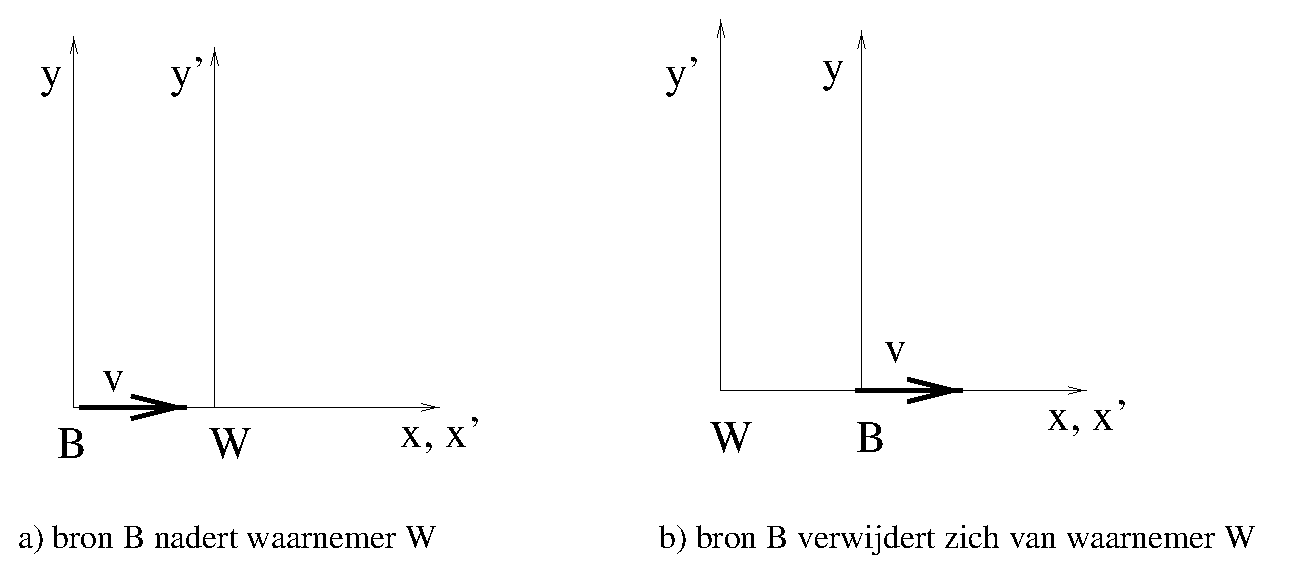
\includegraphics[width=.8\textwidth]{oefeningen.pictures/doppler}
\caption{Bewegende bronnen}
\label{f:doppler}
\end{figure}

We plaatsen een lichtbron in stelsel $S$ en een waarnemer in
stelsel $S'$ met een onderlinge snelheid $v$ tussen $S$ en $S'$.
De Lorentztransformatie geeft dan aan hoe de energie/frequentie, die de 
waarnemer aan de bewegende lichtbron toekent,
afwijkt van de energie/frequentie voor een stilstaande bron.

Eerst: de bron $B$ nadert de waarnemer $W$ (links in fig \ref{f:doppler}a)
\begin{itemize}
\item [a.]
Wat is de Lorentztransformatie voor impuls en energie voor een overgang van
$S$ naar $S'$?
\item [b.]
Leid hieruit de frequentie voor een naderende lichtbron af.
\item [c.]
Ga na of het Doppler-effect hier tot een hogere of lagere frequentie heeft 
geleid.
\end{itemize}
Nu voor een zich verwijderende bron (rechts in figuur \ref{f:doppler}b).
\begin{itemize}
\item [d.]
Bepaal $E'$ en leid de frequentie voor de zich verwijderende bron af.
\item [e.]
Is $\nu '$ groter of kleiner dan $\nu $?
\item [f.]
In welke van de twee gevallen is er sprake van een `roodverschuiving'?
\end{itemize}

%%%%%%%%%%%%%%
\subsection{Roodverschuiving}
In het uitdijend heelal verwijderen veraf gelegen sterrenstelsels zich van ons
af met een snelheid $v$ die toeneemt met hun afstand $d : v \approx Hd$ 
($H$ is de Hubble constante).
Deze verwijdering valt af te lezen uit de `roodverschuiving' van bekende 
spectraallijnen, die nu een grotere golflengte $\lambda '$ dan de 
gebruikelijke $\lambda$ hebben.

De roodverschuiving wordt beschreven door de parameter 
$z = \frac{\lambda ' - \lambda}{\lambda}$.
\begin{itemize}
\item [a.]
Laat zien dat $z = \sqrt{\frac{1 + \beta}{1 - \beta}} -1$.
\item [b.]
Schets een grafiek van $z$ tegen $\beta$.
\end{itemize}
Voor melkwegstelsels op een afstand $d = 10^{8}$   lichtjaar is 
$z \approx 10^{-2}$.
Voor quasars op een afstand $d = 10^{10}$ lichtjaar is $z \approx 1$.
\begin{itemize}
\item [c.]
Maak met deze gegevens een schatting van de Hubble-constante.
\item [d.]
Bereken $\frac{1}{H}$ en laat zien dat deze van de orde van de ouderdom van het heelal is.
\end{itemize}

%%%%%%%%%%%%%%%
\subsection{Stoplicht}
Hoe hard moet je rijden om een stoplicht, dat op rood staat, als een groen
stoplicht te zien?
De golflengte van rood licht is 700 nm, die van groen licht 500 nm.

%%%%%%%%%%%%%%
\subsection{Transversaal Doppler-effect}
In stelsel $S$ staat een waarnemer $W$ ergens op de positieve $y$-as en 
beweegt een lichtbron $B$ zich met snelheid $v$ naar rechts langs 
de $x$-as. We kijken naar de lichtstraal die $B$ in de richting van $W$ 
uitzendt als $B$ op $t=0$ de oorsprong van $S$ passeert (dus een 
foton dat zich langs de positieve $y$-as beweegt, 
met impuls $p_{y}=\frac{E}{c}=\frac{h\nu}{c}$).
\begin{itemize}
\item [a.]
Geef de Lorentztransformatie voor de energie-impuls viervector tussen 
stelsel $S$ en het ruststelsel $S'$ van de lichtbron 
(de stelsels vallen samen op $t=t'=0$).
\item [b.]
Teken de lichtstraal van $B$ naar $W$ in $S'$. Loopt die schuin naar 
{\it linksboven} of naar {\it rechtsboven}?
\item [c.]
In $S$ geldt voor het foton: $p_{x}=0$.
Maak hiervan gebruik om een relatie tussen $E$ en $E'$ voor het foton af te 
leiden en laat zien dat hieruit voor de frequentie van het licht volgt:  
$\nu= \nu '\sqrt{1-\beta ^{2}}$
\item [d.]
In $S'$ wijst de impulsvector van het foton schuin naar linksboven, 
met componenten $p'_{x}$  en  $p'_{y}$.
Laat met de stelling van Pythagoras en de Lorentztransformatie zien dat 
ook in $S'$ geldt:  $|p'|=\frac{E'}{c}$.
\item [e.]
Is er in dit geval sprake van een Doppler-effect (hoewel de lichtbron geen 
snelheidscomponent naar de waarnemer heeft)?
\item [f.]
Is dit `transversale' Doppler-effect groter of kleiner dan het Doppler-effect 
van een naderende of zich verwijderende lichtbron?
\item [g.]
De niet-relativistische Doppler-formule voor een naderende lichtbron is:

\begin{eqnarray}
\nu_{D_{L+}} &=& \frac{c}{c-\nu}\nu = \frac{1}{1-\beta}\nu ;   \\
 \mathrm{en\ }  \nu_{D_T} &=& \nu \  \mathrm{(voor\ 
een\ transversaal\ bewegende\ lichtbron).} \nonumber
\end{eqnarray}

Laat zien dat het relativistische Doppler-effect gelijk is aan het `niet-relativistische Dopper effect gecombineerd met tijddilatatie'.
\end{itemize}



\subsection{Tweelingparadox}
Op Nieuwjaarsdag 2010 vertrekt een astronaut A van de aarde met
snelheid $\beta=0.8$, om naar de dichtsbijzijnde ster, $\alpha$-centauri te gaan. Deze ster staat 4 lichtjaren weg, gemeten in het
coordinatenstelsel verbonden met de aarde. Nadat A de ster heeft
bereikt, keert hij onmiddelijk om en keert terug naar aarde met
dezelfe snelheid, om aan te komen op Nieuwjaarsdag 2020 (aardse
tijd). De astronaut heeft een broer B die achterblijft op aarde, en ze
spreken af elkaar elk jaar op Nieuwjaarsdag een radiobericht te sturen totdat
de reiziger terug is.
\begin{enumerate}
\item Laat zien dat A 6 boodschappen stuurt (inclusief die op de dag van aankomst) terwijl B 10 boodschappen verstuurt.
\item Teken een ruimte-tijd diagram van de reis van A in aardse co\"{o}rdinaten. Teken ook de wereldlijnen van de 
boodschappen die B verstuurd. Laat met dit diagram zien dat A slechts 1 bericht heeft ontvangen op het moment dat hij omkeert,
en dat hij er vervolgens 9 ontvangt tijdens de tweede helft van zijn reis.
\item
Teken een nieuw ruimte-tijd diagram, weer in aardse co\"{o}rdinaten, en teken daarin de wereldlijnen van de astronaut en al de
berichten die {\it hij} verstuurt. Laat zien dat zijn broer op aarde elke 3 jaar een bericht ontvangt gedurende de eerste 9 jaar en dan
3 tijdens het laatste jaar: een totaal van 6.
\item Interpreteer deze resultaten in termen van het Doppler-effect.

\end{enumerate}




